\documentclass[a4paper,11pt]{article}
\usepackage[top=2cm,bottom=2cm,left=2cm,right=2cm]{geometry}
\usepackage[utf8]{inputenc}
\usepackage[frenchb]{babel}

\usepackage{multirow}
\usepackage{makecell}
\usepackage{fancyhdr}
\usepackage{caption}
\usepackage[final]{pdfpages}
\usepackage{tikz,pgfplots,pgf}
\usepackage{subcaption}
\usepackage{siunitx}
\usepackage[toc,page]{appendix}
\usepackage{tcolorbox, listings} 
\usepackage{sectsty}
\usepackage[french]{minitoc} 
\usepackage{hyperref}
\usepackage{colortbl}
\usepackage{mwe}
\usepackage{amsmath}
\usepackage{lipsum}

\definecolor{Pantone2377C}{HTML}{2C5574}
\definecolor{subtitlecolour}{HTML}{00A2A9}
\definecolor{codegreen}{rgb}{0,0.6,0}
\definecolor{codegray}{rgb}{0.5,0.5,0.5}
\definecolor{codeblue}{HTML}{3E8BC0}
\definecolor{codeorange}{HTML}{ffa334}
\definecolor{backcolour}{HTML}{efefef}

\lstdefinestyle{myPython}{
    language=Python,
    backgroundcolor=\color{backcolour},   
    commentstyle=\color{codegreen},
    otherkeywords={plt, np, df},
    keywordstyle=\color{codeblue},
    numberstyle=\tiny\color{codegray},
    stringstyle=\color{codeorange},
    basicstyle=\ttfamily\footnotesize,
    breakatwhitespace=false,         
    breaklines=true,                 
    keepspaces=true,                 
    numbers=left,       
    numbersep=5pt,                  
    showspaces=false,                
    showstringspaces=false,
    showtabs=false,                  
    tabsize=2,
    inputencoding=utf8
}

\lstdefinestyle{myLog}{
    language={[latex]TeX},
    backgroundcolor=\color{backcolour},   
    basicstyle=\ttfamily\footnotesize,
    breakatwhitespace=false,         
    breaklines=true,                 
    keepspaces=true,                 
    numbers=left,       
    numbersep=5pt,                  
    showspaces=false,                
    showstringspaces=false,
    showtabs=false,                  
    tabsize=2,
    inputencoding=utf8
}

\lstset{
  backgroundcolor=\color{backgroundColour},   
  commentstyle=\color{codegreen},
  keywordstyle=\color{codeblue},
  numberstyle=\tiny\color{codegray},
  stringstyle=\color{codeorange},
  basicstyle=\footnotesize,
  breakatwhitespace=false,         
  breaklines=true,                 
  captionpos=b,                    
  keepspaces=true,                 
  numbers=left,                    
  numbersep=5pt,                  
  showspaces=false,                
  showstringspaces=false,
  showtabs=false,                  
  tabsize=2,
  literate=
  {é}{{\'e}}1
  {è}{{\`{e}}}1
  {ê}{{\^{e}}}1
  {û}{{\^{u}}}1
  {ù}{{\`{u}}}1
  {â}{{\^{a}}}1
  {à}{{\`{a}}}1
  {ç}{{\c{c}}}1
  {Ç}{{\c{C}}}1
  {ô}{{\^{o}}}1
}


% Entête et pied de page
\pagestyle{fancy}
\rhead{
\includegraphics [scale=0.035]{img/ensta-logo.png}}
\chead{}
\lhead{}
\lfoot{Tanguy ROUDAUT - Tadios QUINIO}
\rfoot{FIPA promotion 2024}
\cfoot{\thepage}
\renewcommand{\headrulewidth}{0.4pt}
\renewcommand{\footrulewidth}{0.4pt}


\title{TP2: Statistiques descriptives bivariées}
\author{Tanguy ROUDAUT — Tadios QUINIO \and FIPASE 24}
\date{13 Septembre 2022}

\begin{document}

\maketitle

\section{Statistiques descriptives bivariées sur des données d’Iris}
\subsection{Étude de la largeur du pétale en fonction de la longueur du pétale}
\subsubsection*{Représentation graphique}
\vspace{.2cm}

%%%%%
\noindent
\textbf{Question~1~:} Tracer le nuage de points de la longueur du pétale en fonction de la largeur du pétale
pour les 150 iris contenus dans les données ((numpy.)plot, (numpy.)scatter). Ne pas oublier de
mettre des titres sur les axes. Décrire le nuage de points.
\vspace{.2cm}


\begin{figure}[!h]
    \centering
    \begin{minipage}{.60\linewidth}
        \begin{center}
            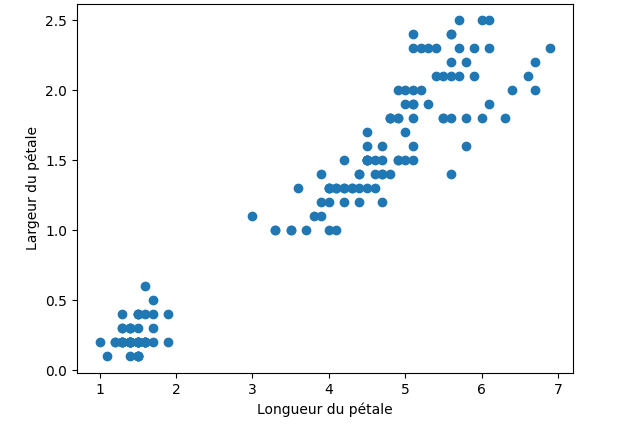
\includegraphics[width=1\textwidth]{img/Figure_1.png}
            \caption{\label{fig:figure1}Nuage de points de la longueur en fonction de la largeur du pétale des 150 Iris}
        \end{center}
    \end{minipage}\hfill
    \begin{minipage}{.36\linewidth}
        Dans un premier temps, on remarque deux concentrations principale. \\
        La première a une longueur de pétale qui varie entre 1~cm et 2~cm pour une largeur d’environ 0,2~cm et 0,6~cm. La seconde, une longueur variant de 3~cm à 7~cm avec une largeur de 
        1~cm à 2,5~cm. \\

        \noindent
        On constate également que la longueur de pétale varie proportionnellement à la largeur.
    \end{minipage}
\end{figure}

\begin{lstlisting}[style=myPython, caption=Code Python pour calculer le coefficient de corrélation, frame=lines]
plt.scatter(petallength, petalwidth)
plt.ylabel("Largeur du pétale")
plt.xlabel("Longueur du pétale")
plt.title("Nuage de points de la longueur en fonction de la largeur du pétale")
plt.show()
\end{lstlisting}

\clearpage

%%%%%
\noindent
\textbf{Question~2~:} Rappeler la définition du coefficient de corrélation et le calculer par la fonction ((numpy.)corrcoef)
\vspace{.2cm}

Le coefficient de corrélation est une valeur qui permet de déterminer s'il existe une relation linéaire entre deux variables, ce qui veut dire que si ces variables sont corrélées alors elles sont liées. \\


\begin{lstlisting}[style=myPython, caption=Code Python pour calculer le coefficient de corrélation, frame=lines]
corr_coef_matrix = np.corrcoef(petallength, petalwidth)
print("Matrice de corrélation:\n",corr_coef_matrix)
\end{lstlisting}

\begin{lstlisting}[style=myLog, caption=Résultat du code, frame=lines]
Matrice de corrélation:
[[1.        0.9627571]
[0.9627571 1.       ]]
\end{lstlisting}

\vspace{.5cm}


%%%%%
\noindent
\textbf{Question~3~:} Donner l’équation de la droite de régression linéaire, créer une fonction permettant de la
calculer à partir de deux variables X et Y et tracer la sur le même graphique
\vspace{.2cm}

\begin{enumerate}
    \item \textbf{Résultat et analyse~:}
        \begin{figure}[!h]
            \centering
            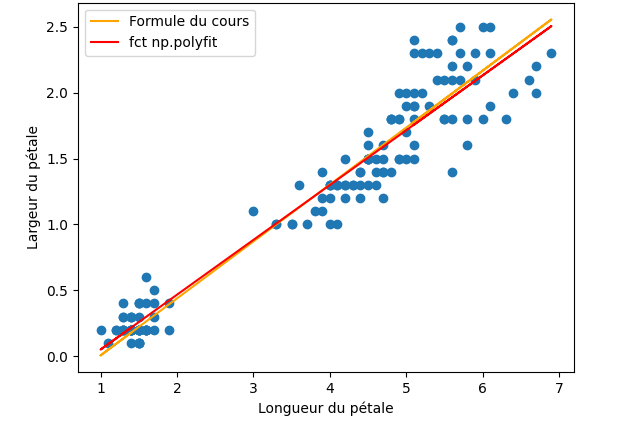
\includegraphics[width=.6\textwidth]{img/Figure_2.png}
            \caption{\label{fig:figure2}Équation de la droite de régression linéaire sur le nuage de points}
        \end{figure}

    \item \textbf{Formules utilisées~:}
        \begin{gather}
            \hat{a} = \rho_{X,Y}.\frac{S_{n-1,Y}}{S_{n-1,X}} \qquad \text{et} \qquad \hat{b} = \overline{Y_{n}}.\rho_{X,Y}.\frac{S_{n-1,Y}}{S_{n-1,X}}.\overline{X_{n}}
        \end{gather}

        \vspace{.5cm}

    \item \textbf{Code python~:}
        \begin{lstlisting}[style=myPython, caption=Code Python pour tracer la droite de régression linéaire, frame=lines]
# Méthode par la formule du cours
def regression_lineaire(corr_coef, x, y):
    mean_x = np.mean(x)
    var_x = np.var(x)
    e_type_x = np.sqrt(var_x)

    mean_y = np.mean(y)
    var_y = np.var(y)
    e_type_y = np.sqrt(var_y)

    a = corr_coef * (e_type_y/e_type_x)
    b = mean_y - corr_coef * ((e_type_y/e_type_x)) * mean_x

    return a, b


a, b = regression_lineaire(corr_coef, petallength, petalwidth)

# Méthode avec polyfit de numpy
fit = np.polyfit(petallength, petalwidth, 1)
poly = petallength*fit[0]+fit[1]

plt.plot(petallength, a*petallength+b, color='orange', label='Formule du cours')
plt.plot(petallength, poly, color='red', label='fct np.polyfit')
plt.scatter(petallength, petalwidth)
plt.ylabel("Largeur du pétale")
plt.xlabel("Longueur du pétale")
plt.title("Equation de la droite de régression linéaire")
plt.legend()
plt.show()
        \end{lstlisting}
    
    \vspace{.2cm}
\end{enumerate}









\vspace{.5cm}


%%%%%
\noindent
\textbf{Question~4~:} Analyser le lien entre les deux variables
\vspace{.2cm}

On constate que les variables \textit{petalLenght} et \textit{petalWidth} sont liées, elles évoluent proportionnellement l'une avec l'autre. \\
On peut donc soumettre l'hypothèse que ces variables sont corrélées puisqu'il existe deux réels tels que $Y=aX+b$.

\vspace{.3cm}

\subsection{Étude de la longueur de pétale selon les différentes espèces}
\subsubsection*{Représentations graphiques}
\vspace{.2cm}

%%%%%
\noindent
\textbf{Question~5~:} Représenter sur une même figure, les trois histogrammes de la longueur de pétale: un
histogramme pour chaque espèce avec une couleur. Commenter cette figure.
\vspace{.2cm}

\begin{figure}[!h]
    \centering
    \begin{minipage}{.48\linewidth}
        \begin{center}
            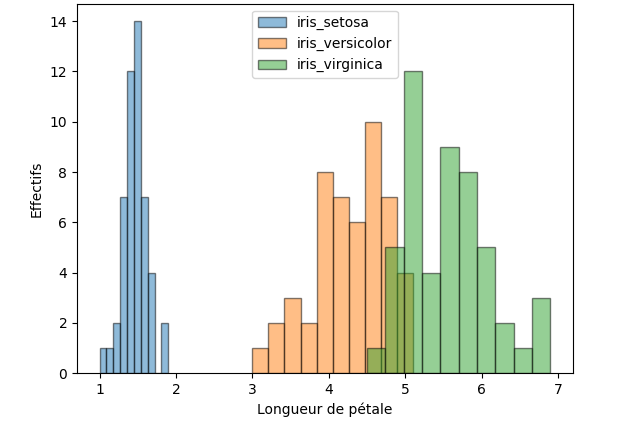
\includegraphics[width=1\textwidth]{img/Figure_3.png}
            \caption{\label{fig:figure3}Histogrammes de la longueur de pétale pour chaque espèce}
        \end{center}
    \end{minipage}\hfill
    \begin{minipage}{.48\linewidth}
        Lors du \textit{TP1 question 7}, nous avions pu remarquer que l'une des espèces a une taille de pétale plus faible, mais qui varie également moins que les deux autres. Le problème était que c'était seulement une hypothèse, puisque nous n'avions pas cette répartition 
        entre les différentes espèces. \\
        L'histogramme de la figure \ref*{fig:figure3}, reprend le même schéma que celui de la \textit{question~7 du TP1}, mais cette fois si en prenant en compte les différentes espèces. \\
        On peut donc conclure que notre hypothèse est vraie, l'iris setosa est plus petite que les deux autres espèces.
    \end{minipage}
\end{figure}

\begin{lstlisting}[style=myPython, caption=Code Python pour calculer le coefficient de corrélation, frame=lines]
iris_setosa_petallength = []
iris_versicolor_petallength = []
iris_virginica_petallength = []

for i in range(len(species)):
    if species[i] == 'Iris-setosa':
        iris_setosa_petallength.append(petallength[i])
    elif species[i] == 'Iris-versicolor':
        iris_versicolor_petallength.append(petallength[i])
    elif species[i] == 'Iris-virginica':
        iris_virginica_petallength.append(petallength[i])

plt.hist(iris_setosa_petallength, edgecolor='black', alpha=0.5, label='iris_setosa')
plt.hist(iris_versicolor_petallength, edgecolor='black', alpha=0.5, label='iris_versicolor')
plt.hist(iris_virginica_petallength, edgecolor='black', alpha=0.5, label='iris_virginica')
plt.xlabel('Longueur de pétale')
plt.ylabel('Effectifs')
plt.title("Histogrammes de la longueur de pétale pour chaque espèce")
plt.legend()
plt.show()
\end{lstlisting}

\vspace{.5cm}


%%%%%
\noindent
\textbf{Question~6~:} Représenter sur une même figure. une boite à moustache par espèce. Commenter cette
figure.
\vspace{.2cm}

\begin{figure}[!h]
    \centering
    \begin{minipage}{.66\linewidth}
        \begin{center}
            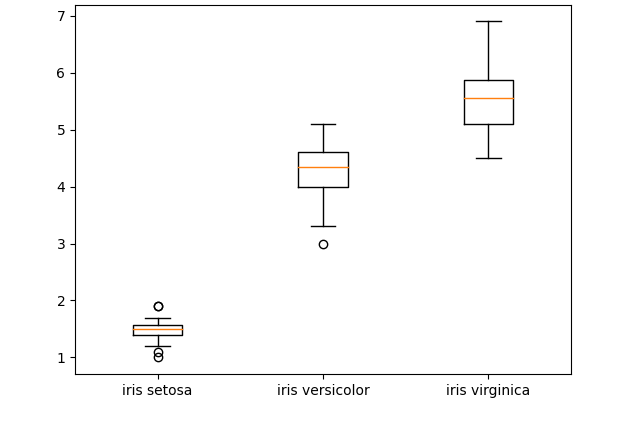
\includegraphics[width=1\textwidth]{img/Figure_4.png}
            \caption{\label{fig:figure4}Boite à moustache de la longueur de pétale pour chaque espèce}
        \end{center}
    \end{minipage}\hfill
    \begin{minipage}{.30\linewidth}
        On remarque encore une fois que l'iris setosa à un intervalle de longueur de pétales plus faible que les deux autres espèces.
    \end{minipage}
\end{figure}

\begin{lstlisting}[style=myPython, caption=Code Python pour calculer le coefficient de corrélation, frame=lines]
boxplot_petallength = [iris_setosa_petallength, iris_versicolor_petallength, iris_virginica_petallength]
plt.boxplot(boxplot_petallength, labels=['iris setosa', 'iris versicolor', 'iris virginica'])
plt.title("Boite à moustache de la longueur de pétale pour chaque espèce")
plt.show()
\end{lstlisting}

\clearpage

\subsubsection*{Représentations graphiques}
\vspace{.2cm}

%%%%%
\noindent
\textbf{Question~7~:} Calculer le rapport de corrélation lié à la décomposition de la variance en variance intraclasse et interclasse. Qu’en concluez-vous?
\vspace{.2cm}

\begin{enumerate}
    \item \textbf{Formules utilisées~:}
        \begin{figure}[!h]
            \centering
            \begin{minipage}{.49\linewidth}
                \begin{itemize}
                    \item[--] Variance interclasse~: 
                        \begin{equation}
                            S^2_{B} = \frac{1}{n} \sum_{i=1}^{p} n_{i}(\overline{Y_{i}} - \overline{Y})^2
                        \end{equation}
                \end{itemize}
            \end{minipage}\hfill\vline
            \begin{minipage}{.49\linewidth}
                \begin{itemize}
                    \item[--] Variance intraclasse~:
                        \begin{equation}
                            S^2_{W} = \frac{1}{n} \sum_{i=1}^{p} n_{i}.S^2_{n-1,Y_{i}}
                        \end{equation}
                \end{itemize}
            \end{minipage}
        \end{figure}

        \begin{itemize}
            \item[--] Variance totale~:
                \begin{equation}\label{eq:var_total}
                    S^2_{n-1,Y} = S^2_{B} + S^2_{W}
                \end{equation}
            \item[--] Rapport de corrélation~:
                \begin{equation}
                    S_{\frac{Y}{X}} = \sqrt{\frac{S^2_{B}}{S^2_{n-1,Y}}} \in [0 , 1]
                \end{equation}
        \end{itemize}

    \item \textbf{Valeurs obtenues~:}
    
        \vspace{.2cm}

        \begin{center}
            \begin{tabular}{| c | c |}
                \hline
                \textbf{Variance interclasse} & 2.910\\\hline
                \textbf{Variance intraclasse} & 0.181\\ \hline
                \textbf{Variance total} & 3.092\\ \hline
                \textbf{Rapport de corrélation} & 0.970\\ \hline


            \end{tabular}
        \end{center}

        \vspace{.5cm}

    \item \textbf{Conclusion~:}
    
        \vspace{.2cm}
        
        La variance totale trouvée grâce à la formule \ref*{eq:var_total}, correspond avec celle trouvée avec \textit{numpy}. Cette constatation nous permet de nous assurer que nos résultats sont corrects et de trouver par la suite le rapport 
        de corrélation qui est de 0,970. \\
        Le rapport de corrélation étant proche de 1 nous permet de confirmer notre hypothèse établie à la \textit{question~4} concernant la corrélation des variables \textit{petalLength} et \textit{petalWidth}.

        \vspace{.5cm}

    \item \textbf{Code python~:}
    
    \vspace{.2cm}

        \begin{lstlisting}[style=myPython, caption=Code Python pour calculer le coefficient de corrélation, frame=lines]
n_cumul = len(species)

mean_species_petallength = [np.mean(iris_setosa_petallength), np.mean(iris_versicolor_petallength), np.mean(iris_virginica_petallength)]

mean_petallength = np.mean(petallength)

var_species_petallength = [np.var(iris_setosa_petallength), np.var(iris_versicolor_petallength), np.var(iris_virginica_petallength)]

n_species = [len(iris_setosa_petallength), len(iris_versicolor_petallength), len(iris_virginica_petallength)]



def var_inter_classe_petallength(n_cumul, n_species, mean_species, mean):
    ret = 0
    for i in range(len(speciesname)):
        ret += n_species[i] * (mean_species[i] - mean)**2

    return ret/n_cumul



def var_intra_classe_petallength(n_cumul, n_species, var_species):
    ret = 0
    for i in range(len(speciesname)):
        ret += n_species[i] * var_species[i]

    return ret / n_cumul



var_inter_classe = var_inter_classe_petallength(n_cumul, n_species, mean_species_petallength, mean_petallength)

var_intra_classe = var_intra_classe_petallength(n_cumul, n_species, var_species_petallength)

var_totale_formule = var_inter_classe + var_intra_classe

var_totale = np.var(petallength)

rapport_corr = np.sqrt(var_inter_classe/var_totale_formule)

print("Variance interclasse: ", var_inter_classe)
print("Variance intraclasse: ", var_intra_classe)
print("Variance total trouvé avec la formule: ", var_totale_formule)
print("Variance total trouvé avec numpy: ", var_totale)
print("Rapport de corrélation: ", rapport_corr)
            \end{lstlisting}
            
            \begin{lstlisting}[style=myLog, caption=Résultat du code, frame=lines]
Variance interclasse:  2.910958222222223
Variance intraclasse:  0.1814666666666667
Variance total trouvé avec la formule:  3.0924248888888894
Variance total trouvé avec numpy:  3.092424888888889
Rapport de corrélation:  0.9702159417163924                
            \end{lstlisting}


\end{enumerate}




\clearpage
\section{Code complet}
\begin{lstlisting}[style=myPython, caption=Code Python complet TP3, frame=lines]
from scipy import stats
import numpy as np

# question 1
x = np.array([0.82, 0.87, 0.77, 0.96, 0.75, 0.83, 0.87, 0.81])
xn = np.mean(x)
ecart_type_x = np.std(x, ddof=1)
n = len(x)
ic = 95
alpha = 1 - ic / 100
t = stats.t.ppf(1 - (alpha / 2), n - 1)

I = xn - (t * ecart_type_x) / np.sqrt(n)
u = xn + (t * ecart_type_x) / np.sqrt(n)

I = round(I, 3)
u = round(u, 3)

print("Question 1:\n", "Borne inférieur:", I, "\n", "Borne supérieur:", u, end="\n\n")

# question 2
x = np.array([0.84, 0.87, 0.89, 0.73, 0.84, 0.81, 0.88, 0.85, 0.89, 0.79, 0.79, 0.90,
              0.59, 0.75, 0.67, 0.76, 0.86, 0.88, 0.70, 0.75, 0.81, 0.77, 0.83, 0.84, 
              0.71, 0.78, 0.59, 0.91, 0.74, 0.68, 0.77, 0.66, 0.80, 0.74, 1.02, 0.91,
              0.55, 0.84, 0.66, 0.77])
p = np.mean(x)
ecart_type_x = np.std(x, ddof=1)
n = len(x)
ic = 95
alpha = 1 - ic / 100
z = stats.norm.ppf(1 - (alpha / 2), loc=0, scale=1)

borne_inf = p - z * (ecart_type_x/np.sqrt(n))
borne_supp = p + z * (ecart_type_x/np.sqrt(n))

borne_inf = round(borne_inf, 3)
borne_supp = round(borne_supp, 3)

print("Question 2:\n", "Borne inférieur:", borne_inf, "\n", "Borne supérieur:", borne_supp, end="\n\n")

# question 3
n = 1000
n_dupond = 500
n_durand = 250
n_duroc = 50

def intervalle_confiance(n, x, ic ):
    p = x/n
    alpha = 1 - ic / 100
    z = stats.norm.ppf(1 - (alpha / 2), loc=0, scale=1)
    borne_inf = p - z * (np.sqrt(p*(1-p)/n))
    borne_supp = p + z * (np.sqrt(p*(1-p)/n))

    return round(borne_inf, 3), round(borne_supp, 3)

borne_inf_dupond_95, borne_supp_dupond_95 = intervalle_confiance(n, n_dupond, 95)
borne_inf_durand_95, borne_supp_durand_95 = intervalle_confiance(n, n_durand, 95)
borne_inf_duroc_95, borne_supp_duroc_95 = intervalle_confiance(n, n_duroc, 95)
borne_inf_dupond_99, borne_supp_dupond_99 = intervalle_confiance(n, n_dupond, 99)
borne_inf_durand_99, borne_supp_durand_99 = intervalle_confiance(n, n_durand, 99)
borne_inf_duroc_99, borne_supp_duroc_99 = intervalle_confiance(n, n_duroc, 99)

print("Question 3:")
print(" Dupond")
print("\t --> Borne inférieur à 95%:", borne_inf_dupond_95)
print("\t --> Borne supérieur à 95%:", borne_supp_dupond_95)
print("\t\t\t ------------------------")
print("\t --> Borne inférieur à 99%:", borne_inf_dupond_99)
print("\t --> Borne supérieur à 99%:", borne_supp_dupond_99)
print(" Durand")
print("\t --> Borne inférieur à 95%:", borne_inf_durand_95)
print("\t --> Borne supérieur à 95%:", borne_supp_durand_95)
print("\t\t\t ------------------------")
print("\t --> Borne inférieur à 99%:", borne_inf_durand_99)
print("\t --> Borne supérieur à 99%:", borne_supp_durand_99)
print(" Duroc")
print("\t --> Borne inférieur à 95%:", borne_inf_duroc_95)
print("\t --> Borne supérieur à 95%:", borne_supp_duroc_95)
print("\t\t\t ------------------------")
print("\t --> Borne inférieur à 99%:", borne_inf_duroc_99)
print("\t --> Borne supérieur à 99%:", borne_supp_duroc_99, end="\n\n")

# question 4
ic = 95
alpha = 1 - ic / 100
p = 17/100
err = 1/100
z = stats.norm.ppf(1 - (alpha / 2), loc=0, scale=1)
n = (z/err)**2 * p*(1-p)
n = np.ceil(n)

print("Question 4:\n", "Nombre de personne à intérroger:", n, end='\n\n')

# question 5
n_casques = 50
n_dommages = 18
borne_inf_dommages_95, borne_supp_dommages_95 = intervalle_confiance(n_casques, n_dommages, 95)

print("Question 5:")
print(" Casques endommagés")
print("\t --> Borne inférieur à 95%:", borne_inf_dommages_95)
print("\t --> Borne supérieur à 95%:", borne_supp_dommages_95, end="\n\n")

# question 6
ic = 95
alpha = 1 - ic / 100
p = 18/50
err = .02
z = stats.norm.ppf(1 - (alpha / 2), loc=0, scale=1)
n = (z/err)**2 * p*(1-p)
n = np.ceil(n)

print("Question 6:\n", "Nombre de casque à tester:", n, end='\n\n')

# question 7
ic = 95
alpha = 1 - ic / 100
err = .02
z = stats.norm.ppf(1 - (alpha / 2), loc=0, scale=1)
p = np.linspace(0, 1, 101)
n = (z/err)**2 * p*(1-p)
index_n_max = np.where(n == max(n))
n = np.ceil(float(n[index_n_max]))

print("Question 7:\n", "Nombre de casque à tester:", n, end='\n\n')    
\end{lstlisting}



\end{document}